% !TEX root = ../main.tex

\chapter{Method}
\label{ch:method}

\section{Benchmarks in Reinforcement Learning}
\label{sec:benchmarks}
When developing a novel algorithm, it is important to compare our results with existing models. For this evaluation, we need standard benchmark problems. These are a set of standard optimization problems. OpenAI Gym is a toolkit created for exactly this scenario. As mentioned in Section~\ref{sec:gym}, it contains a collection of benchmark problems with various levels of difficulty. However, not all benchmark problems are meaningful for the evaluation of an algorithm. If a problem is too trivial to solve, the results do not reflect the quality of the model adequately. We do not need to put a large amount of effort into the creation of a complex model for an easy-to-solve task.

In the paper \emph{Analyzing Reinforcement Learning Benchmarks with Random Weight Guessing} (\cite{oller_analyzing_2020}), the authors analyze and visualize the complexity of standard RL benchmarks based on score distribution. They tested their approach on the five Classic Control benchmark problems from the OpenAI Gym interface: \verb|CartPole|, \verb|Acrobot|, \verb|Pendulum|, \verb|MountainCar|, and \verb|MountainCarCon-| \verb|tinuous|. Given an RL environment, the authors conducted a fixed series of experiments. For these experiments, they used three neural network architectures ($N_{architectures}=3$): a network without any hidden layers (0 HL, 0 HU), a network with a single hidden layer of 4 units (1 HL, 4 HU), and a network with two hidden layers of 4 units each (2 HL, 4 HU). With these, they cover a variety of network models that are suited to solve the given tasks. The evaluation of the benchmark problems should be as objective as possible and should not include bias in the data. To achieve this, the authors did not include any learning opportunities for the network models. Instead, they chose the network weights i.i.d. from the standard normal distribution $\mathcal{N}(0,1)$ with Random Weight Guessing (RWG). This approach assures randomness and no directed learning. The goal of the paper was not to further analyze the network models but to investigate the benchmark problems themselves. With this in mind, they initialized $10^4$ samples ($N_{samples}=10^4$) with different random weights. The number of samples would be too large for a reasonable learning strategy. However, the large number of samples serves a different purpose than optimizing the results. Instead, the aim is to draw statistical conclusions. Each of these samples of a neural network represents a controller that maps observations to actions in the environment. Later in this thesis, I will explore function approximators other than neural networks representing the controller. In the paper, the authors tested the controllers for each environment during 20 independent episodes ($N_{episodes}=20$). For each episode, they saved the score in the score tensor $S$. Algorithm~\ref{alg:environment-evaluation} illustrates the procedure with pseudocode.

\begin{algorithm}
\caption{Evaluation process taken from \cite{oller_analyzing_2020}}
\begin{algorithmic}[1]
\State Initialize environment
\State Create array $S$ of size $N_{architectures} \times N_{samples} \times N_{episodes}$
\For{$n = 1,2,...,N_{samples}$}
    \State Sample NN weights randomly from $\mathcal{N}(0,1)$
    \For{$e=1,2,...,N_{episodes}$}
      \State Reset the environment
      \State Run episode with NN
      \State Store accured episode reward in $S_{a,n,e}$
    \EndFor
\EndFor
\end{algorithmic}
\label{alg:environment-evaluation}
\end{algorithm}

After the authors obtained the scores, they calculated the mean performance over all episodes from a sample and its variance. These statistics are significant insights. They can reveal how stable the network models are in completing a given task. A low mean value suggests that, in general, the network cannot complete the task. The variance gives us further insight into the score distribution. It illustrates how spread out the scores are from their respective mean score. A high value means that we have high variability. A controller is valuable if it can solve a specific task reliably and stable. Therefore, we strive for a high value for the mean and a low value for the variance. However, training a network with random weight guessing should generally not result in a stable controller. If this is the case, we can assume that the task to solve was too trivial and is not valuable for evaluation measurements. In the illustrations of the paper, the authors ranked the samples according to their mean scores. They then visualized their results with three plots: a log-scale histogram of the mean scores, a scatter plot of the sample scores over their rank, a scatter plot of score variance over the mean score.

I reproduced the results of the authors following the mentioned methodology. My findings for the environment \verb|CartPole| are displayed in Figure~\ref{fig:plots_reproduced}.
\begin{figure}[ht]
\centering
\begin{subfigure}{\textwidth}
  \centering
  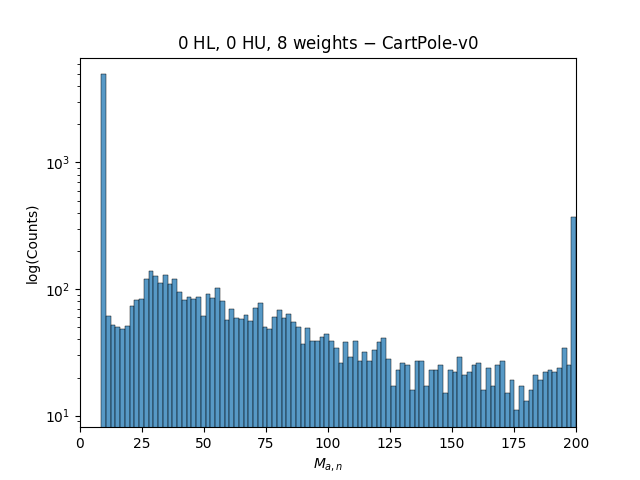
\includegraphics[width=0.329\textwidth]{reproduced_plots/HL_0_HU_0_histogram}
  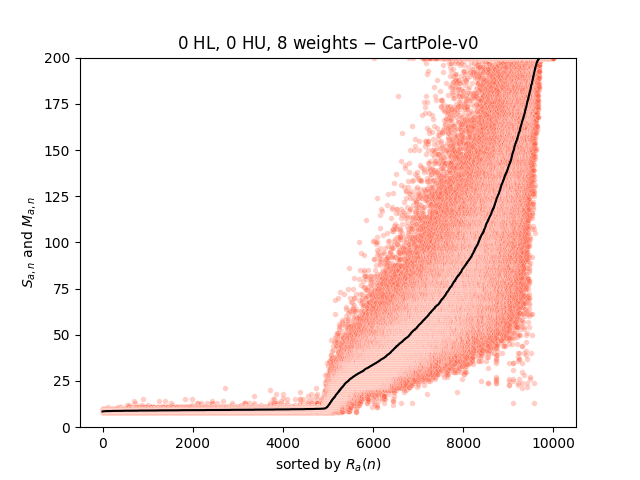
\includegraphics[width=0.329\textwidth]{reproduced_plots/HL_0_HU_0_scatter_score}
  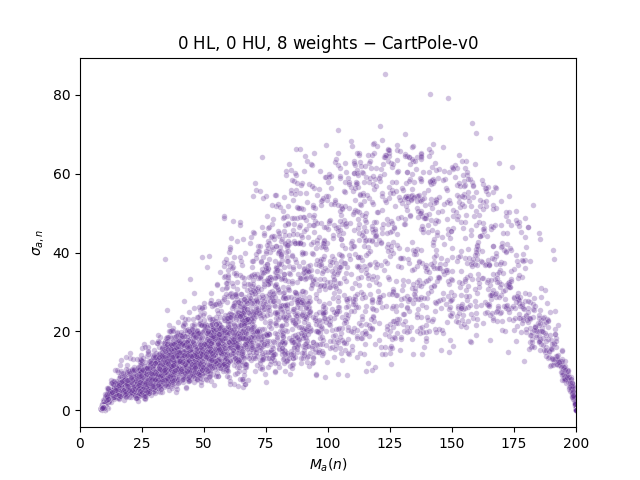
\includegraphics[width=0.329\textwidth]{reproduced_plots/HL_0_HU_0_scatter_sd}
    \caption{Results of network architecture without hidden layers}
    \label{fig:plots_reproduced_first}
\end{subfigure}
\begin{subfigure}{\textwidth}
  \centering
  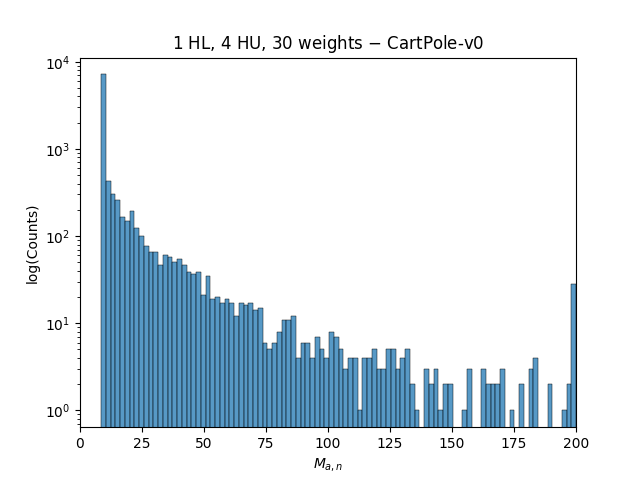
\includegraphics[width=0.329\textwidth]{reproduced_plots/HL_1_HU_4_histogram}
  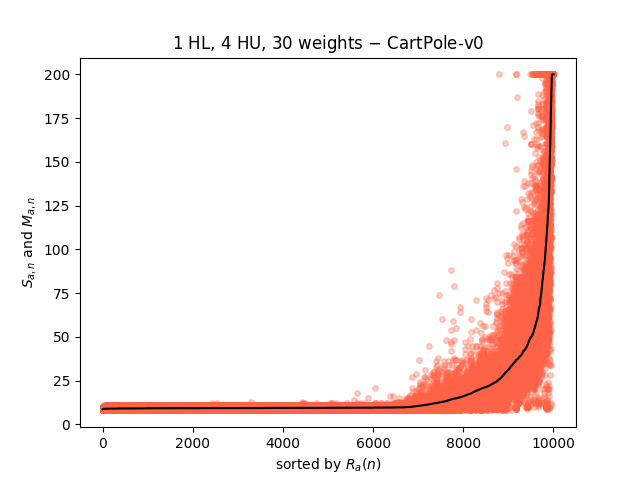
\includegraphics[width=0.329\textwidth]{reproduced_plots/HL_1_HU_4_scatter_score}
  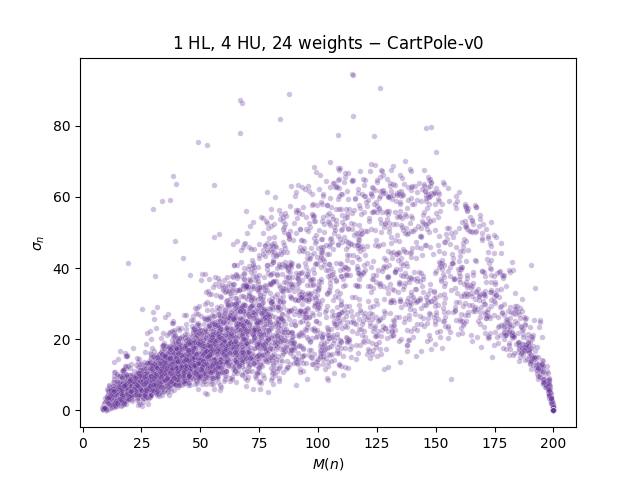
\includegraphics[width=0.329\textwidth]{reproduced_plots/HL_1_HU_4_scatter_sd}
    \caption{Results of network architecture with one hidden layer}
    \label{fig:plots_reproduced_second}
\end{subfigure}
\begin{subfigure}{\textwidth}
  \centering
  \includegraphics[width=0.329\textwidth]{reproduced_plots/HL_2_HU_4_histogram}
  \includegraphics[width=0.329\textwidth]{reproduced_plots/HL_2_HU_4_scatter_score}
  \includegraphics[width=0.329\textwidth]{reproduced_plots/HL_2_HU_4_scatter_sd}
    \caption{Results of network architecture with two hidden layers}
    \label{fig:plots_reproduced_third}
\end{subfigure}
\caption[Reproduced Plots]{
  \textbf{Results of the benchmark evaluation.}
   The plots show a log-scale histogram of the mean scores (left images), a scatter plot of the sample scores over their rank (middle images), a scatter plot of score variance over the mean score (right image). As expected with RWG, most networks were not able to solve the given task. However, there is still a significant amount of samples achieving a mean score of 200. That suggests that the environment is trivial to solve.
}
\label{fig:plots_reproduced}
\end{figure}
The plots illustrate the results for each of the three network architectures. Each row shows the histogram of the mean score values in the left image, the scatter plot of all scores over their rank in the image in the middle, and the scatter plot of the score variance over the mean score in the right image for a specific network architecture. There are few differences, but overall all network architectures deliver similar insights. The histogram plots show that the majority of networks receive a low score. Since the weights of the networks were chosen with RWG, this is rather unsurprising. But there is still a significant amount of networks that were able to achieve a high mean value or even the maximum value of 200. With a score of 200, the network was able to solve the task each episode. Therefore, the network could reliably solve the task without any learning technique involved. This should not be the case for a complex task. Furthermore, in the scatter plot in the middle, we can see that the line plot of the mean scores is a continuous increasing line without any jumps. Thus, a suited RL algorithm should generally be able to learn the task incrementally without converging into a local optimum. At the top of the scatter plot, we can see quite a few data points with a score of 200 that have a relatively low mean score. This indicates that a network that generally performs poorly can still solve the task with the right initialization conditions. Lastly, in the scatter plot on the right, we can see the distribution of the variance according to the mean value. On the left side, we have low scores of variance corresponding with a low mean value. These networks were consistently unable to achieve a high score. Without any training involved, we can expect most networks to be in this area. However, in the middle of the plot, the data points are spread out. For a high variance, the scores of a network differ highly from the mean value. Thus, we might get lucky and receive a high score depending on initialization conditions, but we might as well get a low score. These networks are inconsistent and unstable. On the right side of the scatter plot, we can see that the data points with a high mean value are mostly of low variance. Thus, to achieve a high mean value, the network needs consistency.

\subsection{Impact of Bias}
Interestingly, the usage of the bias had a relatively large impact on the performance of the network in my experiments. Without bias, the networks seem to achieve overall better scores. All plots in Figure~\ref{fig:plots_reproduced} illustrate the results without bias. For comparison, Figure~\ref{fig:comparison_bias} shows the results of a network with two hidden layers with the same configurations as before but this time including bias. As we can see, the networks with bias connections have a much lower score in general. The number of networks that can consistently solve the task also decreases significantly. In the paper, the authors noted that the probability mass of top-performers generally increases when dropping the bias connections for all tested environments. Thus, this is not an isolated observation. However, they did not investigate this behavior further as it was not the focus of their paper.
\begin{figure}[ht]
\centering
\includegraphics[width=0.329\textwidth]{with_bias_nn/HL_2_HU_4_histogram}
\includegraphics[width=0.329\textwidth]{with_bias_nn/HL_2_HU_4_scatter_score}
\includegraphics[width=0.329\textwidth]{with_bias_nn/HL_2_HU_4_scatter_sd}
\caption[Impact of Bias]{
  \textbf{Impact of bias.}
  The figures show the performance of a network with two hidden layers with the same settings as before but here we include bias. We can clearly see that the network with bias connection performs much worse than the one without.
}
\label{fig:comparison_bias}
\end{figure}
One possible explanation could be that guessing additional weights might be fatal for achieving a good score. Or in other words: the more possibilities we have to falsely guess a weight, the higher the probability to fail. To test this hypothesis, we can alter the number of weights and compare the results. With an increased number of weights, we would expect the networks to perform worse than before. However, it could also be that the number of weights is not as impactful as the complexity of the model in general. Randomly guessing the parameters of a simple model has a higher chance to result in a good (simple) model than guessing the parameters of a more complex model. The complexity of the network architecture gives an upper bound for the function that can be approximated. A network with high complexity maps into a larger search space with more complex functions. Since the size of the search space increases, there are also more possible samples that fail to solve the task. As the paper showed, a simple model is sufficient to solve these environments. A complex model is oversized for our purpose here. Thus, randomly guessing a simple model can yield a model with good performance with enough attempts. However, it is unlikely to randomly guess a complex model that performs well without any training involved. To test this hypothesis, we can increase the complexity of a network by varying the number of hidden layers or the number of neurons in a hidden layer. With increased complexity, we would expect the networks to perform worse than before.

Another interesting aspect would be to inspect the role of the bias in connection with the environments. A simple model is sufficient to solve a simple task. But what if the environment is more difficult to solve? In that case, the undersized complexity would limit us from finding an appropriate solution as the search space is not large enough for this scenario. Therefore, including bias should improve the results.

The experiments following this thought process are described in Chapter~\ref{ch:experiments}.


\todo[inline]{How much should be included here and how much in experiments/visualization? Rename section name?}

\section{OpenAI Gym Environments}
\label{sec:environments}
OpenAI Gym offers five classic control environments ready to use: CartPole, Acrobot, MountainCar, MountainCarContiuous, and Pendulum. The initial state of each environment is stochastic. Out of all environments OpenAI Gym provides, the classic control environments are considered as easier ones to solve. Each environment has an observation and an action space. An agent performs some action from the action space and observes how the environment state changes.

\subsection{CartPole}
The CartPole environment corresponds to the pole-balancing problem formulated in \emph{Neuronlike Adaptive Elements That Can Solve Difficult Learning Control Problems} (\cite{6313077}). A pole is attached to a cart that the agent can move along a one-dimensional track. Fig.~\ref{fig:cartpole} shows one possible state of this problem.
\begin{figure}[!ht]
  \centering
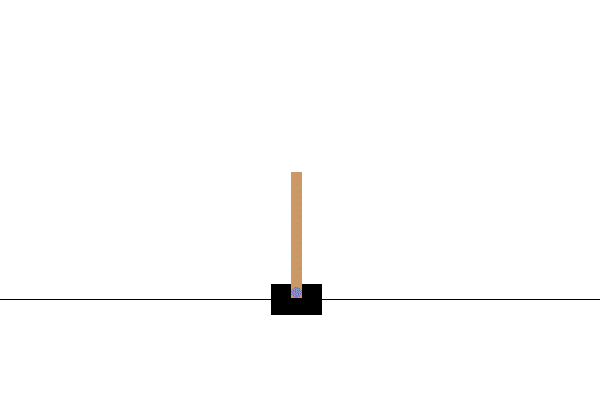
\includegraphics[width=0.5\textwidth]{cartpole}
\caption[Illustration of the environment CartPole]{
  \textbf{Illustration of the environment CartPole.}
  The image shows one possible state of the CartPole environment.
}
\label{fig:cartpole}
\end{figure}
\\
\textbf{Action Space:} The CartPole environment accepts one action per step and has a discrete action space of {0, 1}. The action indicates the direction in which we push the cart by a fixed force. The actions are described in Table~\ref{table:cartpole_act}.
\begin{table}[!ht]
  \centering
  \begin{tabular}{ |c|c| }
    \hline
    Action & Description \\
    \hline
    0 & Push cart to the left \\
    1 & Push cart to the right \\
    \hline
  \end{tabular}
  \caption[Action space of the environment CartPole]{
    \textbf{Action space of the environment CartPole.}
    List of all possible actions for the CartPole environment.
  }
  \label{table:cartpole_act}
\end{table}
\\
\textbf{Observation Space:} For CartPole, we receive four observations that inform us about the position and velocity of the cart as well as the pole. Table~\ref{table:cartpole_obs} shows all observations with the range of the values.
\begin{table}[!ht]
  \centering
  \begin{tabular}{ |c|c|c| }
    \hline
    Observation & Min & Max \\
    \hline
    Cart Position & -4.8 & 4.8 \\
    Cart Velocity & -Inf & Inf \\
    Pole Angle & ~ -0.418 rad (-24°) & ~ 0.418 rad (24°) \\
    Pole Angular Velocity & -Inf & Inf \\
    \hline
  \end{tabular}
  \caption[Observation space of the environment CartPole]{
    \textbf{Observation space of the environment CartPole.}
    Description of all observations for the CartPole environment.
  }
  \label{table:cartpole_obs}
\end{table}
\\
\textbf{Reward:} The goal of this task is to keep the pole upright as long as possible. Thus, we get a positive reward of +1 for each step that does not meet the termination criteria. An episode terminates when either the pole angle is $\pm$12°, the cart position is $\pm$2.4, or the episode length is greater than 200 (500 for v1).

\subsection{Acrobot}
The environment Acrobot is based on the paper \emph{Generalization in Reinforcement Learning: Successful Examples Using Sparse Coarse Coding} (\cite{NIPS1995_8f1d4362}) and the book \emph{Reinforcement Learning: An Introduction} (\cite{montague1999reinforcement}). The system contains a chain with two links, with one end of the chain fixed. The goal is to swing the free end of the chain upwards until a certain height. Fig~\ref{fig:acrobot} shows one possible state for this problem with the fixed height indicated by a horizontal line.
\begin{figure}[!ht]
  \centering
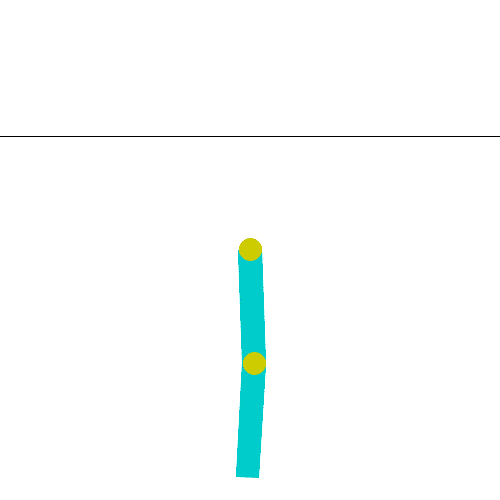
\includegraphics[width=0.5\textwidth]{acrobot}
\caption[Illustration of the environment Acrobot]{
  \textbf{Illustration of the environment Acrobot.}
  The image shows one possible state of the Acrobot environment.
}
\label{fig:acrobot}
\end{figure}
\\
\textbf{Action Space:} For Acrobot, the action space is discrete and deterministic and represents the torque applied to the joint between the two links, including the loose end. Table~\ref{table:acrobot_act} shows a description of all possible actions.
\begin{table}[!ht]
  \centering
  \begin{tabular}{ |c|c|c| }
    \hline
    Action & Description & Unit \\
    \hline
    0 & apply -1 torque to the actuated joint & torque (N m) \\
    1 & apply 0 torque to the actuated joint & torque (N m) \\
    2 & apply 1 torque to the actuated joint & torque (N m) \\
    \hline
  \end{tabular}
  \caption[Action space of the environment Acrobot]{
    \textbf{Action space of the environment Acrobot.}
    List of all possible actions for the CartPole environment.
  }
  \label{table:acrobot_act}
\end{table}
\\
\textbf{Observation Space:} Acrobot returns six observations that inform us about the two rotational joint angles and their angular velocities. Table~\ref{table:acrobot_obs} contains a description for each observation. theta1 is the angle of the first joint, where an angle of 0 indicates the first link is pointing directly downwards. theta2 is relative to the angle of the first link. An angle of 0 corresponds to having the same angle between the two links.
\begin{table}[!ht]
  \centering
  \begin{tabular}{ |c|c|c| }
    \hline
    Observation & Min & Max \\
    \hline
    Cosine of theta1 & -1 & 1 \\
    Sine of theta1 & -1 & 1 \\
    Cosine of theta2 & -1 & 1 \\
    Sine of theta2 & -1 & 1 \\
    Angular velocity of theta1 & ~ -12.567 (-4 * $\pi$) & ~ 12.567 (4 * $\pi$) \\
    Angular velocity of theta2 & ~ -28.274 (-9 * $\pi$) & ~ 28.274 (9 * $\pi$) \\
    \hline
  \end{tabular}
  \caption[Observation space of the environment Acrobot]{
    \textbf{Observation space of the environment Acrobot.}
    Description of all observations for the Acrobot environment.
  }
  \label{table:acrobot_obs}
\end{table}
\\
\textbf{Reward:} The goal is to reach the target height with as little stepts as possible. Thus, each step that does not reach the goal receives a negative reward of -1. Reaching the target height results in a reward of 0. The reward threshold is -100.

\subsection{MountainCar}
For the MountainCar problem, we need to maneuver a car up a hill to its target. For this, we need to strategically accelerate the car to reach the goal. This problem first appeared in Andrew Moore's PhD Thesis \emph{Efficient memory-based learning for
robot control} (\cite{moore1990efficient}). There are two versions of this problem, one with a discrete action space and one with a continuous action space. This version has a discrete action space. Fig~\ref{fig:mountain_car} shows one possible initial state of this environment.
\begin{figure}[!ht]
  \centering
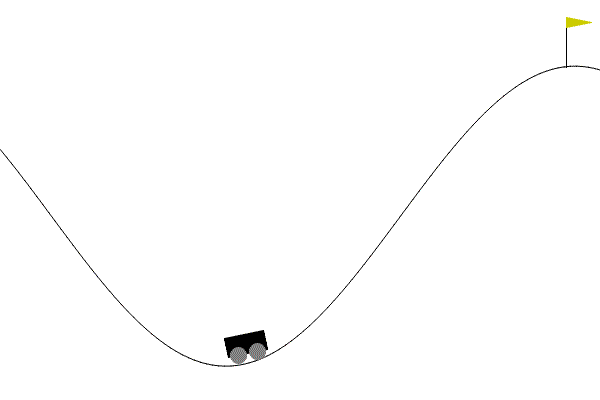
\includegraphics[width=0.5\textwidth]{mountain_car}
\caption[Illustration of the environment MountainCar]{
  \textbf{Illustration of the environment MountainCar.}
  The image shows one possible state of the MountainCar environment.
}
\label{fig:mountain_car}
\end{figure}
\\
\textbf{Action Space:} The action space consists of three discrete actions. We can either accelerate the car to the right or to the left or we do not interact at all. The actions are further described in Table~\ref{table:mountaincar_act}
\begin{table}[!ht]
  \centering
  \begin{tabular}{ |c|c|c|c| }
    \hline
    Action & Description & Value & Unit \\
    \hline
    0 & Accelerate to the left & Inf & position(m) \\
    1 & Don't accelerate  & Inf & position(m) \\
    2 & Accelerate to the right  & Inf & position(m) \\
    \hline
  \end{tabular}
  \caption[Action space of the environment MountainCar]{
    \textbf{Action space of the environment MountainCar.}
    List of all possible actions for the MountainCar environment.
  }
  \label{table:mountaincar_act}
\end{table}
\\
\textbf{Observation Space:} The environment gives us two observations with information about the position and the velocity of the car. They are described in Table~\ref{table:mountaincar_obs}.
\begin{table}[!ht]
  \centering
  \begin{tabular}{ |c|c|c|c| }
    \hline
    Observation & Min & Max & Unit \\
    \hline
    Position of the car along the x-axis & -Inf & Inf & position(m) \\
    Velocity of the car & -Inf & Inf & position(m) \\
    \hline
  \end{tabular}
  \caption[Observation space of the environment MountainCar]{
    \textbf{Observation space of the environment MountainCar.}
    Description of all observations for the MountainCar environment.
  }
  \label{table:mountaincar_obs}
\end{table}
\\
\textbf{Reward:} To solve the environment, the car has to reach the flag on the right hill as fast as possible. For every step in which the agent cannot reach the target, he receives a negativ reward of -1.

\subsection{MountainCarContinuous}
MountainCarContinuous represents the same problem as MountainCar but with a continuous action space.
\\ \\
\textbf{Action Space:} This environment acccepts one continuous action per step. The action represents the directional force on the car and is clipped in the range [-1, 1] and multiplied by a power of 0.0015.
\\ \\
\textbf{Observation Space:} The observation space is the same as in MountainCar. Table~\ref{table:mountaincar_obs} holds the important information.
\\ \\
\textbf{Reward:} Each step in which the car does not reach the target, we receive a negative reward of $-0.1 * action^2$ to penalise actions of large magnitude. If the goal is reached, we receive a positive reward of +100.

\subsection{Pendulum}
In this environment, the system consists of a pendulum attached at one end to a fixed point and the other end being free. The goal is to apply torque on the free end to swing it to an upright position.
\begin{figure}[!ht]
  \centering
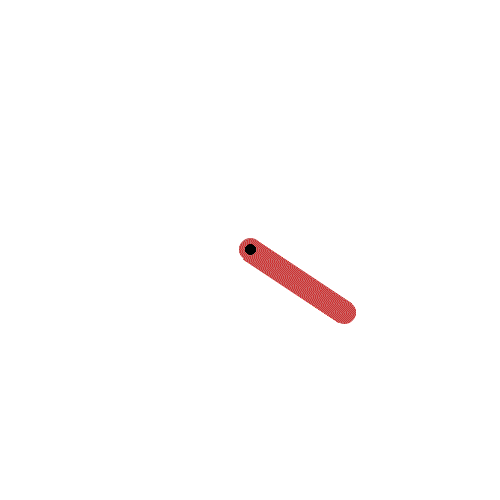
\includegraphics[width=0.5\textwidth]{pendulum}
\caption[Illustration of the environment Pendulum]{
  \textbf{Illustration of the environment Pendulum.}
  The image shows one possible state of the Pendulum environment.
}
\label{fig:pendulum}
\end{figure}
\\
\textbf{Action Space:} The environment accepts one action per step. The action represents the torque applied to the free end of the pendulum.
\begin{table}[!ht]
  \centering
  \begin{tabular}{ |c|c|c|c| }
    \hline
    Action & Description & Min & Max \\
    \hline
    0 & Torque & -2.0 & 2.0 \\
    \hline
  \end{tabular}
  \caption[Action space of the environment Pendulum]{
    \textbf{Action space of the environment Pendulum.}
    List of all possible actions for the Pendulum environment.
  }
  \label{table:pendulum_act}
\end{table}
\\ \\
\textbf{Observation Space:} The environment returns three observations.

\begin{table}[!ht]
  \centering
  \begin{tabular}{ |c|c|c| }
    \hline
    Observation & Min & Max \\
    \hline
    x = cos(theta) & -1.0 & 1.0 \\
    y = sin(angle) & -1.0 & 1.0 \\
    Angular Velocity & -8.0 & 8.0 \\
    \hline
  \end{tabular}
  \caption[Observation space of the environment Pendulum]{
    \textbf{Observation space of the environment Pendulum.}
    Description of all observations for the Pendulum environment.
  }
  \label{table:pendulum_obs}
\end{table}

\todo[inline]{talk about difficulty / what the environment tests, check if versions are correct, not happy with presentation of this section}

\section{Visualization}
For the visualization of the results, I am using similar plots as \cite{oller_analyzing_2020}. The type of plots I will be using are already presented in Figure~\ref{fig:plots_reproduced}. However, I will mainly be using the scatter plots shown in the middle.
\todo[inline]{Rethink paper section, present plots here for the first time?}

\section{Alternative Models}
\label{sec:models}
We can represent many problems in machine learning as a function mapping an input space into an output space. The output space or \textit{search space} denotes the space of all feasible solutions. The underlying function is the output of the learning process of an algorithm and is often called the \textit{target function}. Optimally, we would derive the formula of the function explicitly. However, even though we suspect that such a function exists, we usually do not have enough information to derive a formula directly. Thus, we aim to approximate the target function with \textit{function approximators} by using the available data. In general, we can apply any function approximator. However, each function approximator has its advantages and limitations. For example, some may be prone to local optimum. Depending on the task, this could prevent us from finding a good solution.
\subsection{Polynomials}
In mathematics, a polynomial is the sum of powers in one or more variables multiplied by constant coefficients. Given a field $F$, a polynomial in variable $x$ with coefficients in $F$ is a formal expression denoted by
\begin{align*}
  &f(x) = \Sigma_{i=0}^{n} a_i x^i \in F[x], &a_0, ..., a_n \in F, \ \ i \in \mathbb{N},
\end{align*}
where $F[x]$ represents the set of all such polynomials (\cite{fischer2014}, p. 61). The above formula shows the one dimensional case. For the multi-dimensional case, $x$ and the coefficients are vectors instead of scalars. Thus, a polynomial $p(\mathbf{x})$ with $\mathbf{x} = [x_0, ..., x_m]^T$ being a vector and of degree $n$ can be represented by
\begin{align*}
  &p(\mathbf{x}) = \Sigma_{i=0}^{n} \mathbf{w_i}^T (x_k^i)_{k \in I} \in F^n[\mathbf{x}], &\mathbf{w_0}, ... \mathbf{w_n} \in F^n, \ \ I = \{0, ..., m\}.
\end{align*}
Polynomials are relatively simple mathematical expressions and offer some significant advantages: their derivative and indefinite integral are easy to determine and are also polynomial. Due to their simple structure, polynomials can be valuable to analyze more complex functions using polynomial approximations. \textit{Taylor's theorem} tells us that we can locally approximate any $k$-times differentiable function by a polynomial of degree $k$. We call this approximation \textit{Taylor polynomial}. Furthermore, the \textit{Weierstrass approximation theorem} says that we can uniformly approximate every continuous function defined on a closed interval by a polynomial. Other applications of polynomials are \textit{polynomial interpolation} and \textit{polynomial splines}. Polynomial interpolation describes the problem of constructing a polynomial that passes through all given data points. Polynomial splines are piecewise polynomial functions that can be used for spline interpolation.

For the experiments with a polynomial model in Chapter~\ref{ch:experiments}, I used two architectures $P_1$ and $P_2$. The first model $P_1$ consists of one polynomial for each possible action in a discrete action space. The input of the model is the observation from the environment. The dimension of the weight vectors is according to the dimension of the input vector. For the environment \verb|CartPole| with the discrete action space $\{0, 1\}$ and observation $\mathbf{x} = [x_0, x_1, x_2, x_3]^T$, this means that $P_1$ consists of two polynomials:
\begin{align*}
  &p_0(\mathbf{x}) = \Sigma_{i=0}^{n} \mathbf{w_i}^T (x_k^i)_{k \in I} \in \mathbb{R}, &\mathbf{w_0}, ..., \mathbf{w_3}, \mathbf{x} \in \mathbb{R}^4, \ \ I = \{0, 1, 2, 3\} \\
  &p_1(\mathbf{x}) = \Sigma_{i=0}^{n} \mathbf{\hat{w}_i}^T (x_k^i)_{k \in I} \in \mathbb{R}, &\mathbf{\hat{w}_0}, ..., \mathbf{\hat{w}_3}, \mathbf{x} \in \mathbb{R}^4, \ \ I = \{0, 1, 2, 3\}
\end{align*}
In the formulas, $n$ denotes the degree of the polynomial. In my experiments, I tested polynomials of degrees 1, 2, and 3. The output of the polynomials has no reasonable upper and lower limit, as illustrated in Figure~\ref{fig:bounds}. That makes it harder to interpret the results reasonably.
\begin{figure}[ht]
\centering
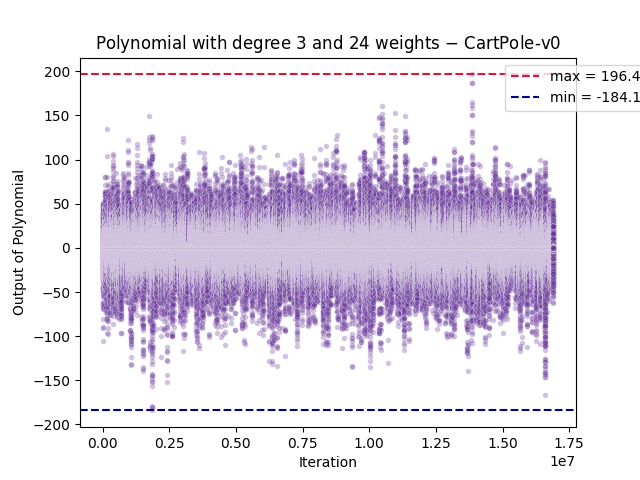
\includegraphics[width=0.6\textwidth]{PolynomialNN_degree_3_bounds}
\caption[Upper and lower bound]{
  \textbf{Upper and lower bound.}
  The figure shows each output of the polynomial functions described above. As we can see, the functions are not well bound, and there are quite a few outliers. That makes it hard to interpret the output sensibly.
}
\label{fig:bounds}
\end{figure}
So, I scaled the outputs with a sigmoid function. A sigmoid function is a mathematical function that maps an arbitrary input space into an output space with a small range, for example, 0 and 1. The function has a characteristic S-shaped curve. We can interpret the output space of the sigmoid function as a probability. In this case, we search for the probability that a specific action is the reasonable one given an observation $\mathbf{x}$. Thus, for our example with the \verb|CartPole| environment, we can interpret $sig(p_0)$ as the probability that action 0 is the correct one and $sig(p_1)$ as the probability that action 1 is the correct one. Putting this thought into a formula for $P_1$ and the \verb|CartPole| environment, we get:
\[
  P_1(\mathbf{x}) =
  \begin{cases}1~&{\text{ if }}~sig(p_1(\mathbf{x})) > sig(p_0(\mathbf{x}))~,\\0~&~\text{otherwise}~.\end{cases}
\]
For the sigmoid function, I used the logistic sigmoid function. The formula and a plot of the function in 2D are shown in Figure~\ref{fig:sigmoid}.
\begin{figure}[ht]
\centering
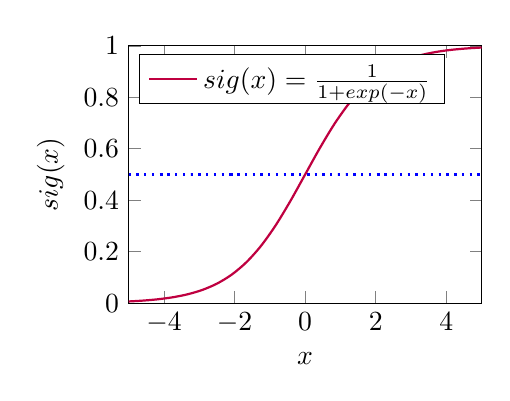
\begin{tikzpicture}
\begin{axis}[
      xmin = -5, xmax = 5,
      ymin = 0, ymax = 1,
      legend cell align = {left},
      legend pos = north west,
      width = 0.5\textwidth,
      height = 0.4\textwidth,
      xlabel = \(x\),
      ylabel = {\(sig(x)\)}
    ]
    \addplot[
        smooth,
        thick,
        purple
    ] {1 / (1 + exp(-x))};
    \addlegendentry{
    $sig(x) = \frac{1}{1 + exp(-x)}$
    }
    \addplot[
        smooth,
        thick,
        blue,
        dotted
    ] {0.5};
\end{axis}
\end{tikzpicture}
\caption[Sigmoid function]{
  \textbf{Sigmoid function.}
  The figure shows a plot of the logistic sigmoid function. The function maps an arbitrary input space into the range between 0 and 1. The output of the function can be interpreted as a probability. It is useful to scale data into a meaningful value.
}
\label{fig:sigmoid}
\end{figure}

The second model $P_2$ is constructed similarly to $P_1$, but it only consists of one polynomial instead of one for each possible action. For the \verb|CartPole| environment, this means $P_2$ consists of:
\[
  p(\mathbf{x}) = \Sigma_{i=0}^{n} \mathbf{w_i}^T (x_k^i)_{k \in I} \in \mathbb{R}, \ \ \ \ \ \ \ \ \ \ \mathbf{w_i} \in \mathbb{R}^4, \ \ I = \{0, 1, 2, 3\}
\]
Analogous to $P_1$, I tested the polynomial $p(\mathbf{x})$ with degrees 1, 2, and 3. So, $n \in \{1, 2, 3\}$. In addition, I again used the logistic sigmoid function to scale the output of the polynomial. However, the output of $P_2$ is determined by a fixed threshold instead of comparing multiple polynomials. Putting this into a formula for the \verb|CartPole| environment, we get:
\[
  P_2(\mathbf{x}) =
  \begin{cases}1~&{\text{ if }}~sig(p(\mathbf{x}))>0.5~,\\0~&~\text{otherwise}~.\end{cases}
\]

\todo[inline]{Include theorems (Taylor, Weierstass) \\ Explain difference between approximation and interpolation \\ Does $F^n$ make sense?}

\subsection{Splines}
General splines, adjustments \\ \\
Splines can also be used as function approximators. However, with splines we do not aim to approximate the whole function but rather return a piecewise approximation.

\todo[inline]{First was sind splines, dann herleitung in this case}


\subsection{Binary Trees}
A binary tree is a fairly simple data structure in computer science. A binary tree consists of nodes that each have at most two children, referred to as left child and right child.
\todo[inline]{Herleitung von splines erklären -> vielleicht in vorheriger subsection?}
